\section{Implementation} % (fold)
\label{sec:implementation}


\begin{table}[h]
	\centering
	\begin{tabular}{r|lll}
	 & \acs{spb} & \acs{mpls} & OpenFlow / \acs{sdn}\\
	\hline
	Tagging of VPN Traffic & \acs{pbb} & \acs{vpls} & \acs{pbb} / \acs{mpls}\\
	MAC Scalability & yes & yes & yes\\
	Topology Discovery & \acs{isis} & \acs{ospf} & application\\
	Path Provisioning & \acs{spt} & \acs{rsvp} / \acs{ldp} & application\\
	Traffic Engineering & limited & \acs{rsvp} & application\\
	\ac{ecmp} & limited & yes & yes, using Groups\\
	\ac{bum} limiting & dependent on \acs{hw} & dependent on \acs{hw} & yes, using Metering\\
	Exchange \acsp{cmac} & no & E-VPN (draft) & application\\
	Traffic Rate Limiting & dependent on \acs{hw} & dependent on \acs{hw} & yes, using Metering\\
	Fast Failover & no & \acs{frr} & yes, using Groups\\
	\acs{oam} & 802.1ag & \acs{lsp} Ping & application\\
	\hline
	Forwarding Decision & \acs{pbb} tags & \acs{mpls} labels & flow entry \\
	\ac{bum} traffic handling & flood & flood & sent to controller\\
	\end{tabular}
	\caption{Required features and corresponding available technologies.}
	\label{tb:reqs}
\end{table}


\begin{figure}[!h]
	\centering
	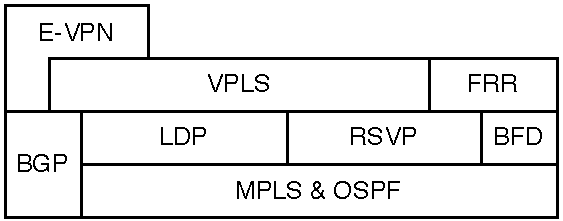
\includegraphics[width=8cm]{./includes/mpls-stack.pdf}
	\caption{Dependency stack of \ac{mpls}-related technologies.}
	\label{fig:mpls-stack}
\end{figure}

Table of protocols

MPLS - tag of traffic
VPLS - encapsulates Ethernet frames
RSVP - distributes labels downstream / ecmp / te
LDP - distributes labels upstream / ecmp
OSPF - learns topology of network
BFD - provide connectivity checks

FRR depends on RSVP
RSVP depends on OSPF

LDP depends on VPLS
VPLS depends on RSVP and MPLS
RSVP depends on OSPF and MPLS

BGP depends on E-VPN
E-VPN depends VPLS
VPLS depends on RSVP
RSVP depends on OSPF and MPLS

depends all on MPLS forwarding plane

PBB - tag traffic
IS-IS - learns topology of network
SPB - ecmp / te

rate limiting, vendor specific

what can provide what function for DVPNs?

\subsection{Contemporary Technologies} % (fold)
\label{sub:contemporary_technologies}

% subsection contemporary_technologies (end)

\subsection{OpenFlow} % (fold)
\label{sub:openflow}

% subsection openflow (end)

% section implementation (end)